\documentclass[12pt]{article}
    
    % LANGUAGE PACKAGES
\usepackage[T1]{fontenc}
\usepackage[utf8]{inputenc}
\usepackage[portuguese]{babel}


	% OTHER PACKAGES
\usepackage[margin=1in]{geometry}
\usepackage[none]{hyphenat}
\usepackage{fancyhdr}
\usepackage{capt-of}
\usepackage{graphicx,calc}
\usepackage{graphics}
\usepackage{float}
\usepackage{indentfirst}

	% HEADER AND FOOOTER
\pagestyle{fancy}
\fancyhead{}
\fancyfoot{}
\fancyhead[L]{\slshape \MakeUppercase{Projeto SD}}
\fancyhead[R]{\slshape Sistemas Digitais 2021.2}
\fancyfoot[C]{\thepage}
\setlength{\headheight}{52pt}
\renewcommand{\footrulewidth}{0pt}


	% CONTENT
\begin{document}
\begin{titlepage}
\begin{center}
\vspace*{1cm}
\Large{\textbf{Sistemas Digitais 2021.2}\\Professor: Stephan Michael Blawid}\\
\vfill
\line(1,0){400}\\[1mm]
\huge{\textbf{Projeto 2}}\\[3mm]
\Large{Relatório do projeto proposto pela disciplina}\\[1mm]
\line(1,0){400}
\vfill
\begin{figure}[!htb]
    \centering
    \includegraphics[scale=0.2]{imgs/logo cin-ufpe.png}\\
    \label{fig:logo}
\end{figure}
Por Yves Emmanuel, David Londres, Natan Frederico e Clesson Roberto\\27 de Agosto de 2021
\end{center}
\end{titlepage}

\setcounter{page}{1}

\section*{Q1}

\subsection*{Resumo}

Esse projeto propõe a elaboração dos circuitos de um micro-ondas através da combinação dos circuitos combinacionais e sequenciais vistos até aqui na disciplina. Um micro-ondas funciona basicamente transmitindo ondas (energia em transição) que excitam as moléculas de água dos alimentos (quanto mais excitadas, maior a temperatura).


Quatro componentes formam a base desse sistema: um transformador que altera a intensidade da corrente elétrica, um diodo que permite a passagem da corrente elétrica em um sentido, um capacitor que armazena cargas elétricas quando submetido à uma tensão e um magnetron que é utilizado para gerar ondas de rádio curtas de acordo com o fluxo de elétrons (corrente elétrica). Aplicando uma potência de corrente alternada de 120 (VAC) no transformador, o micro-ondas é ligado e a passagem da corrente elétrica influenciada por ele e pelo magnetron gera as ondas necessárias para aquecer o alimento. Além disso, um contador é utilizado para determinar o fim do tempo de aquecimento.


Os sinais de entrada do sistema são: um clock para definir o tempo desejado de  funcionamento, um botão para iniciar o funcionamento, um botão para cessar o funcionamento, um botão para zerar o tempo de funcionamento, um sinal interno que indica se a porta está fechada e nove botões para os dígitos númericos (0-9) que introduzem o tempo de funcionamento desejado.


O funcionamento é simples:

\begin{center}
	\begin{itemize}
		\item Quando não está em funcionamento, você pode selecionar o tempo de cozimento desejado, sendo cada dígito anterior ao selecionado deslocado para a esquerda, gerando possíveis valores de segundos e minutos;
		\item Quando o botão iniciar for pressionado, se a porta estiver fechada, o micro-ondas é ligado e o tempo de cozimento decresce em minutos e segundos;
		\item Se a porta for aberta, ou o botão de cessar for pressionado, o micro-ondas é desligado mantendo o valor atual no clock;
		\item Ao pressionar o botão que zera o clock, o micro-ondas é desligado independente do estado, e o tempo atual vai para 0.
	\end{itemize}
\end{center}

Os sinais de saída do sistema são: um sinal que ativa o magnetron, e três sinais que ativam o tempo em minutos, dezenas de segundos e unidades de segundos.


\subsection*{a)} Os blocos funcionais do nível 2 são: o \textit{timer} de minutos/segundos, a entrada/controle do \textit{timer}, o controle de saída do magnetron e o \textit{decoder}/\textit{driver} de 7 segmentos.

\subsection*{b)} O \textit{clock} para o temporizador deve ser uma onda de 1Hz, quando nenhum botão está sendo pressionado.

\subsection*{c)} Quando qualquer botão estiver sendo pressionado, então um sinal de 100Hz deve ser direcionado para o temporizador.


\section*{Q2}

\subsection*{Mux 2 para 1)} O teste ocorreu da forma esperada, não houve nenhum problema de execução, visto que é um módulo muito simples.

\subsection*{Latch SR)}  Foram atribuídos diversos valores para S e R, a saída Q obteve resultados consistentes com a tabela da veradade do latch SR.



\subsection*{Contador mod 6 e mod 10)} 


\section*{Q3}

\subsection*{Decodificador)} Foram testados os dois estados para as três unidades de tempo: unidades de segundos, dezenas de segundos e unidades de minutos. A entrada recebia valores entre 0 e 1, saída obteve os valores esperados, ou 7E ou 30 – em hexadeximal – respectivamente.


\subsection*{Magnetron)} O magnetron funciona conforme esperado, sendo ativado no nível baixo da variável \textit{start}, contanto, é necessário que a porta esteja fechada para a ativação da saída. A saída também funciona para a entrada \textit{clear}, desativando o magnetron de acordo.

\subsection*{Temporizador)} Tivemos dificuldade em gerar a onda do comportamento do temporizador. Apesar de termos atribuído valores às entradas, a onda não foi gerada.

\section*{Q4}

\subsection*{Microondas)} No primeiro teste, colocamos o microondas para esquentar durante 3 minutos e 59 segundos. O teste foi um sucesso, o microondas só ligava quando a porta estava fechada.

No segundo teste, colcamos o microondas para esquentar durante 2 minutos e 45 segundos. Além disso, interrompemos a execução do microondas, e depois o colocamos para esquentar novamente. O módulo funcionou quando esperado, parando de esquentar quando a porta foi aberta.

\section*{Q5}
\subsection*{Primeiro caso teste)} 

\begin{figure}[!htb]
    \centering
    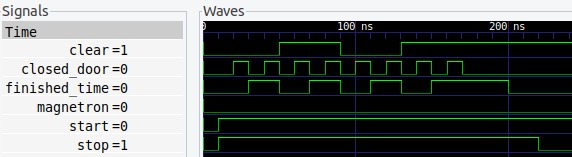
\includegraphics[scale=0.7]{imgs/testecontrol1}\\
    \label{fig:teste1}
\end{figure}

Note que até pouco mais de 200 ns, o magnetron não inicia pois nos instantes em que \textit{finished\underline{ }time = 0} , isto é, o término do cozimento não está finalizado, a porta do microondas está aberta, isto é, \textit{closed\underline{ }door = 0}. Além disso, nos instantes em que a porta está de fato fechada, o \textit{clear = 1}, isto é, o tempo de cozimento é resetado, logo em nenhum desses instantes o magnetron tem sinal 1.

\subsection*{Segundo caso teste)} 

\begin{figure}[!htb]
    \centering
    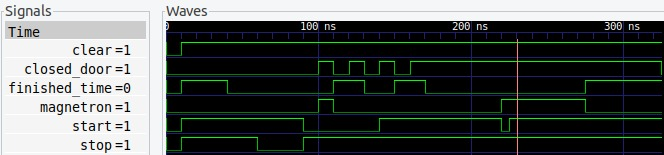
\includegraphics[scale=0.7]{imgs/testecontrol2}\\
    \label{fig:teste2}
\end{figure}

Note que há dois instantes onde o magnetron é ativado, e ele obedece as condições necessárias: a porta do microondas está fechada e o tempo de cozimento não acabou, isso é, \textit{closed\underline{ }door = 1} e \textit{finished\underline{ }time = 0}.


\pagebreak
\section*{Q6}
\begin{center}
\textbf{Autoavaliação}
\end{center}

O projeto foi muito difícil de executar, eram muitos componentes separados e ainda tínhamos de nos preocupar em juntá-los no nível 2 e no nível 1. Os testes realizados funcionam como esperado, o responsável por fazer os testes da questão 2 na \textit{testbench} não conseguiu terminar e relatar o seu trabalho.

Faltou um pouco de coordenação dentro da equipe, mas isso já era esperado, visto que nunca trabalhamos juntos antes. Além disso, o projeto coincidiu com as últimas avaliações do período, diminuindo nossa atenção.
Acredito que nosso projeto vale 8 numa escala de 0 a 10.

\end{document}
